\chapter{Produktspezifikationen}
Dieses Kapitel behandelt die Planung und Spezifikation des Projekts.
Weiteres wird die verwendete Technologieauswahl begründet und mit Alternativlösungen verglichen.

\section{Anforderungen und Spezifikationen}
Hier kommt noch was über Anforderungen und Spezifikatioinen

\subsection{Use Cases}
Hier kommt noch was über Use Cases

\section{Design}
Hier kommt noch was über das Design

\subsection{Abläufe}
Hier werden die Abläufe der drei Szenarien modeliert und eingefügt
\begin{figure}[H]
    \centering
    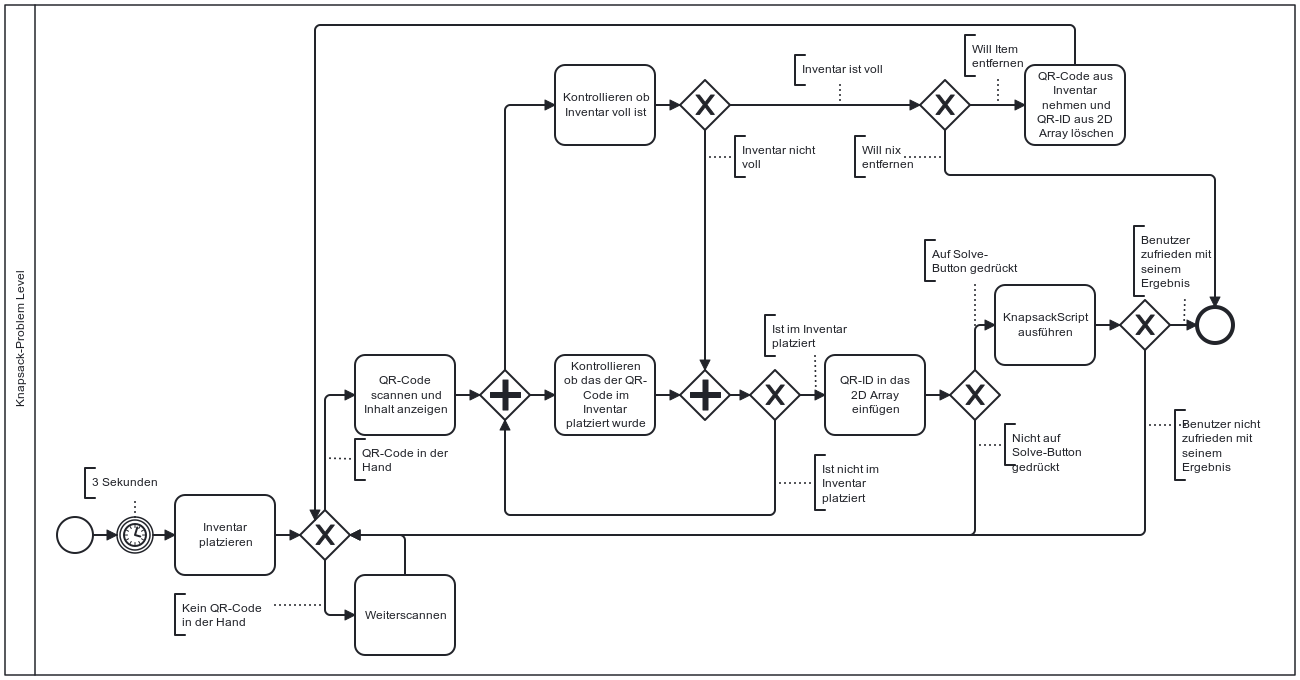
\includegraphics[scale=0.5, angle=270]{images/AblaufdiagrammLevel2}
    \caption{Ablaufdiagramm des Knapsack-Problem Levels}
    \label{fig:Ablaufdiagramm Level 2}
\end{figure}

\section{Eingesetzte Technologien}

\subsection{Kriterien}
Bei der Auswahl der eingesetzten Technologien war es von besonderer Bedeutung, dass diese möglichst zuverlässig und
bereits etabliert sind. Die ausgewählten Technologien sollten eine hohe Ausfallsicherheit gewährleisten, einfach zu
bedienen sein und vor allem eine performante Nutzung der Applikation sicherstellen.

\subsection{Game Engine}\marginpar{\small\(\rightarrow\) SKREPEK}
Um einen reibungslosen Verlauf des Projekts zu gewährleisten, ist die sorgfältige Auswahl der richtigen Game Engine von
entscheidender Bedeutung. Die Game Engine fungiert als fundamentale Plattform für die Entwicklung und Erstellung von
Videospielen, indem sie eine umfassende Palette von Werkzeugen, Bibliotheken und Funktionen bereitstellt, die Entwicklern
helfen, Spiele zu konzipieren, zu gestalten und zu optimieren. In diesem Abschnitt werden zwei potenzielle Game Engines,
die für das Projekt in Betracht gezogen wurden, eingehend untersucht und anschließend die Gründe für die getroffene Auswahl
erläutert.

\subsubsection{Unity}
Unity ist eine Game Engine, die von Entwicklern weltweit für die Erstellung von 2D- und 3D-Spielen genutzt wird. Sie
unterstützt verschiedene Plattformen wie PC, Konsolen, Mobilgeräte und AR/VR-Geräte. Unity bietet Entwicklern eine
umfangreiche Sammlung von Werkzeugen und Ressourcen, um Spiele schnell zu prototypen und zu entwickeln.

Ein herausragendes Merkmal von Unity ist der Asset Store. Hier können Entwickler Assets wie 3D-Modelle, Texturen, Sounds
und Plugins kaufen oder verkaufen. Dadurch können sie ihre Projekte mit hochwertigen Inhalten erweitern und verbessern,
ohne alles von Grund auf neu erstellen zu müssen. Unity bietet außerdem eine starke Community-Unterstützung mit Foren,
Tutorials und Schulungen, was besonders für neue Entwickler hilfreich ist.

Die Programmierung in Unity erfolgt hauptsächlich durch die Verwendung von C# als Skriptsprache. Diese ist sowohl für
erfahrene Entwickler als auch für Anfänger zugänglich. Unity ist aufgrund der Kombination von benutzerfreundlichen Werkzeugen,
einer großen Community und einer breiten Plattformunterstützung eine beliebte Wahl für Indie-Entwickler sowie für große Studios.

\subsubsection{Unreal Engine}
Die Unreal Engine ist eine leistungsstarke Game Engine, die für ihre hochwertigen Grafiken und fortgeschrittenen Funktionen
bekannt ist. Sie wird häufig für die Entwicklung von AAA-Titeln sowie für hochwertige VR-Erfahrungen verwendet. Die Engine
bietet branchenführende Grafikfunktionen wie fortschrittliche Beleuchtung, Partikelsysteme, Physiksimulationen und Echtzeit-Rendering.

Eine bemerkenswerte Funktion der Unreal Engine ist das Blueprints-System. Es ermöglicht Entwicklern, Spiele und interaktive
Inhalte ohne herkömmlichen Programmiercode zu erstellen. Dadurch wird die Engine besonders zugänglich für Künstler und
Designer, die möglicherweise keine tiefen Programmierkenntnisse haben.

Die Unreal Engine bietet eine umfangreiche Sammlung von vorgefertigten Assets und Werkzeugen sowie einen integrierten
Marketplace, auf dem Entwickler zusätzliche Inhalte erwerben können. Sie unterstützt eine Vielzahl von Plattformen,
darunter PC, Konsolen, Mobilgeräte und VR-Headsets.

Insgesamt ist die Unreal Engine eine leistungsstarke Wahl für Entwickler, die hochwertige Grafiken und fortschrittliche
Funktionen in ihren Spielen und Anwendungen benötigen. Sie wird häufig von größeren Studios genutzt, die Zugang zu hochwertigen
Tools und Support benötigen.

\subsubsection{Game Engine Auswahl und Wechsel im Projektverlauf}
Bei Projektbeginn wurde nach umfassender Recherche und Evaluierung verschiedener Optionen entschieden, die Unreal Engine
als primäre Entwicklungsumgebung für dieses Projekt zu verwenden. Diese Entscheidung wurde aufgrund mehrerer überzeugender
Faktoren getroffen, darunter insbesondere das beliebte Blueprint-Scripting-System, das die Entwicklung von interaktiven
Inhalten erleichtert und auch für Personen ohne umfangreiche Programmierkenntnisse zugänglich macht. Zusätzlich zu diesem
herausragenden Merkmal wurden weitere Aspekte berücksichtigt, die die Unreal Engine zu einer attraktiven Wahl machten,
wie beispielsweise ihre leistungsstarken Grafikfunktionen, die branchenweit anerkannt sind, sowie ihre Unterstützung für
die Entwicklung hochwertiger VR-Erfahrungen und AAA-Titel.

\subsubsection*{Herausforderungen im ersten Monat des Entwicklungsprozesses}
Trotz der zu Beginn getroffenen Entscheidung für die Unreal Engine traten im Verlauf des ersten Monats des Entwicklungsprozesses
bestimmte Herausforderungen auf. Diese Herausforderungen können als unerwartete Schwierigkeiten betrachtet werden, die während
der Umsetzung des Projekts auftraten und möglicherweise die ursprüngliche Entscheidung beeinflussen könnten. Im Einzelnen
wurden folgende Herausforderungen identifiziert:
\begin{enumerate}
    \item \textbf{Mangelhafte Dokumentation für AR-Entwicklung in der Unreal Engine:} Die unzureichende Dokumentation
    für die Entwicklung von Augmented Reality (AR)-Anwendungen in der Unreal Engine erwies sich als erhebliche Hürde.
    Fehlende detaillierte Anleitungen und Referenzen für AR-spezifische Funktionen behinderten die effiziente Integration von AR-Elementen.
    \item \textbf{Begrenzte Verfügbarkeit von AR-spezifischen Online-Tutorials:} Ein Mangel an Online-Tutorials,
    die sich speziell mit der Entwicklung von AR-Anwendungen in der Unreal Engine befassten, führte zu einer
    beträchtlichen Lernkurve für das Entwicklerteam und verzögerte den Implementierungsprozess von AR-spezifischen Features.
    \item \textbf{Komplexität der AR-Entwicklung in der Unreal Engine:} Die Unreal Engine erwies sich als
    anspruchsvoller in Bezug auf die Umsetzung von AR-spezifischen Funktionen. Die Notwendigkeit, komplexe Skripte zu
    erstellen und vielfältige Einstellungen anzupassen, führte zu einem erhöhten Zeitaufwand für die Umsetzung von AR-Elementen.
    \item \textbf{Mangelhafte Integration von AR-spezifischen Werkzeugen:} Schwächen in der Integration von
    AR-spezifischen Entwicklungswerkzeugen in der Unreal Engine erschwerten eine nahtlose Interaktion mit AR-Plattformen
    und die optimale Nutzung ihrer Funktionen.
    \item \textbf{Eingeschränkte Community-Unterstützung für AR-Entwicklung:} Im Vergleich zu Unity war die Community-Unterstützung
    für die AR-Entwicklung in der Unreal Engine begrenzt. Die Verfügbarkeit von Ratschlägen und Lösungen für spezifische
    AR-Herausforderungen war eingeschränkt, was die Eigenständigkeit bei der Lösung von Problemen beeinträchtigte.
\end{enumerate}

Diese Herausforderungen bildeten die Grundlage für die strategische Entscheidung des Projektteams, von der Unreal Engine
zu Unity zu wechseln. Der Wechsel ermöglichte eine effizientere und zielführende Entwicklung der AR-Applikation,
gestützt durch Unity's umfassende Unterstützung, detaillierte Dokumentation und breite Community-Ressourcen.

\subsection{Unity foundation packages}\marginpar{\small\(\rightarrow\) SKREPEK}
Um Augmented Reality (AR)-Applikationen in Unity erfolgreich zu entwickeln, sind bestimmte \textit{Foundation Packages}
erforderlich. Diese Pakete müssen in Unity importiert werden, um grundlegende Funktionalitäten bereitzustellen, die für
die erfolgreiche Umsetzung einer AR-Applikation notwendig sind. Im Folgenden werden die beiden wesentlichen Pakete näher
erläutert, die für die Funktionalität einer solchen Applikation unerlässlich sind.

\subsubsection{MRTK3}
Das Mixed Reality Toolkit 3 (MRTK3) ist ein leistungsstarkes Open-Source-Entwicklungstoolkit, das von Microsoft entwickelt
und gepflegt wird. Es ist speziell darauf ausgerichtet, die Entwicklung von Mixed-Reality-Anwendungen zu erleichtern,
indem es eine umfassende Sammlung von Komponenten, Skripten und Assets bereitstellt. MRTK3 bietet Entwicklern eine Vielzahl
von Funktionen und Werkzeugen, die speziell für die Erstellung von Anwendungen für Augmented Reality (AR), Virtual Reality
(VR) und Mixed Reality (MR) optimiert sind.

Das Toolkit umfasst eine breite Palette von Funktionen, darunter Interaktionselemente wie Hand- und Gestenerfassung,
räumliches Mapping, Physiksimulationen für Objekte in der realen Welt, Benutzerschnittstellen-Design-Werkzeuge und vieles
mehr. MRTK3 ist plattformübergreifend und unterstützt verschiedene AR-/VR-Headsets sowie andere Mixed-Reality-Geräte.

Die Bedeutung von MRTK3 für die Entwicklung von AR-Applikationen liegt in seiner Fähigkeit, Entwicklern eine solide
Grundlage und eine Vielzahl von vordefinierten Komponenten und Tools zu bieten, die den Entwicklungsprozess beschleunigen
und vereinfachen. Durch die Verwendung von MRTK3 können Entwickler komplexe AR-Anwendungen schneller prototypisieren und
implementieren, da sie auf eine umfangreiche Bibliothek von Funktionen zugreifen können, die speziell für AR-Szenarien
optimiert sind. Dies erhöht die Effizienz der Entwicklung und ermöglicht es den Entwicklern, sich auf die Gestaltung und
Umsetzung innovativer AR-Erfahrungen zu konzentrieren, ohne sich um die Grundlagen der AR-Entwicklung kümmern zu müssen.\footnote{Microsoft Dokumentation \cite{Mixed Reality Toolkit 3}}

\subsubsection{Microsoft OpenXR Plugin}
Das Microsoft OpenXR Plugin stellt eine bedeutende Komponente im Kontext der Entwicklung von Augmented Reality (AR)-Applikationen
innerhalb der Unity-Entwicklungsumgebung dar. Entwickelt und bereitgestellt von Microsoft, ermöglicht dieses Plugin die
nahtlose Integration des OpenXR-Standards in Unity. OpenXR, initiiert durch die Khronos Group, fungiert als branchenweiter
Standard zur Vereinheitlichung der XR-Anwendungsentwicklung, wobei XR für Extended Reality steht und sowohl Augmented
Reality (AR), Virtual Reality (VR) als auch Mixed Reality (MR) umfasst.

Das Microsoft OpenXR Plugin erleichtert Entwicklern die Arbeit innerhalb von Unity, indem es eine reibungslose Integration
des OpenXR-Standards ermöglicht. Hierdurch erhalten Entwickler Zugang zu einer breiten Palette von Funktionen und
Möglichkeiten, die durch den OpenXR-Standard standardisiert sind, inklusive plattformübergreifender Kompatibilität sowie
optimierter Leistung für XR-Anwendungen.

Die Relevanz des Microsoft OpenXR Plugins für die AR-Entwicklung liegt in seiner Fähigkeit, eine konsistente Entwicklungsumgebung
für XR-Anwendungen innerhalb von Unity zu schaffen. Durch die Nutzung dieses Plugins können AR-Entwickler die Vorteile
des OpenXR-Standards voll ausschöpfen, einschließlich verbesserte Kompatibilität, Leistung und Zukunftssicherheit ihrer Anwendungen.

Zusätzlich erlaubt das Plugin den Entwicklern den Zugriff auf spezifische Funktionen und Optimierungen, die von Microsoft
speziell für die AR-Entwicklung entwickelt wurden. Dies beinhaltet beispielsweise Features zur Verbesserung der
AR-Umgebungserkennung, Handhabung von Eingaben sowie Optimierung der Grafikleistung für AR-Anwendungen.\footnote{Khronos Group \cite{OpenXR Plugin}}

\subsubsection{Integrationsprozess der Plugins}
Zur Integration der genannten Plugins, nämlich des \textit{Mixed Reality Toolkit 3} und des \textit{OpenXR Plugin}, in
den Unity Editor wird das externe Tool namens \textit{Mixed Reality Feature Tool} von Microsoft verwendet. Dieses Tool
fungiert als umfassende Sammlung von Plugins und Erweiterungen im Bereich der Augmented und Virtual Reality Entwicklung
für Unity. Neben den erwähnten Plugins umfasst es weitere wichtige Erweiterungen, darunter:
\begin{itemize}
    \item Azure Mixed Reality Services
    \item Experimental
    \item Mixed Reality Toolkit
    \item MRTK3 (Mixed Reality Toolkit 3)
    \item Plattform Support
    \item Spatial Audio
    \item World Locking Tools
    \item Weitere Funktionen (Other features)
\end{itemize}

Um die Integration durchzuführen, müssen innerhalb des \textit{Plattform Support} Bereichs des \textit{Mixed Reality Feature Tools}
sowohl das \textit{Mixed Reality OpenXR Plugin} als auch das gesamte MRTK3-Paket ausgewählt werden. Nach der Auswahl
dieser Pakete ist es erforderlich, sie zu validieren und anschließend in das Unity-Projekt zu importieren.

Dieser Prozess gewährleistet eine erfolgreiche Integration der benötigten Plugins und Erweiterungen, die für die Entwicklung
von Augmented Reality-Anwendungen in Unity von entscheidender Bedeutung sind.

\subsection{Modellierungsprogramm}\marginpar{\small\(\rightarrow\) LAMPEL}

Die Erstellung der 3D-Modelle für die beiden Level erfordert ein Rendering-Programm. Die Entscheidung für das
Rendering-Programm Blender wurde bereits zu Beginn des Projekts getroffen. \\
Diese Wahl basiert auf folgenden Gründen:
\begin{itemize}
    \item \textbf{Kostenfrei und Open Source}\\
    Blender ist kostenfrei und quelloffen, was bedeutet, dass es ohne Lizenzkosten genutzt werden kann. Dies ist
    besonders attraktiv bei der Entwicklung von AR-Anwendungen mit begrenztem Budget.
    \item \textbf{Echtzeit-Rendering}\\
    Blender verfügt über einen Echtzeit-Renderer namens Eevee, der schnelle Vorschauen
    und Renderings ermöglicht. Dies ist hilfreich, um AR-Inhalte in Echtzeit anzuzeigen und zu überprüfen.
    \item \textbf{Integration mit AR-Frameworks}\\
    Obwohl Blender keine direkte Unterstützung für AR-Funktionen bietet, können die erstellten 3D-Modelle und
    Animationen in AR-Entwicklungsumgebungen wie Unity oder Unreal Engine importiert werden, um dort
    AR-spezifische Funktionalitäten hinzuzufügen.
\end{itemize}

\subsubsection{Wie funktioniert Blender im Allgemeinen?}

Die nachfolgende Beschreibung hebt die Schlüsselaspekte und die Funktionalität von Blender für unseren speziellen
Anwendungsbereich hervor.

\begin{itemize}
    \item \textbf{Benutzeroberfläche und Interaktion}\\
    Die Benutzeroberfläche von Blender ist komplex gestaltet, aber hoch anpassbar. Sie enthält 3D-Modelle,
    Ansichten, Fenster und Panels. Benutzer interagieren mit Objekten und Werkzeugen über Maus- und Tastaturbefehle,
    wobei erfahrene Nutzer Hotkeys oder Shortcuts verwenden können, um effizienter zu arbeiten.

    \item \textbf{3D-Modellierung}\\
    Blender ermöglicht die Erstellung von 3D-Modellen durch die Verwendung von Primitiven wie Würfeln, Kugeln,
    Flächen und Kurven. Diese können dann bearbeitet und modifiziert werden, um komplexe Formen zu erstellen.
    Modellierungswerkzeuge umfassen Extrusion, Verschiebung, Skalierung und Rotation.

    \item \textbf{Materialien und Texturen}\\
    Zur Erzeugung realistischer Oberflächen können Materialien erstellt und Texturen auf Objekte angewendet werden.
    Blender erlaubt die Feinanpassung von Materialeigenschaften wie Diffusreflexion, Glanz, Transparenz und Emission.

    \item \textbf{Gemeinschaft und Ressourcen}\\
    Blender verfügt über eine engagierte Benutzergemeinschaft, die umfassende Dokumentation, Tutorials und Foren
    bereitstellt. Diese Ressourcen erleichtern die Einarbeitung und die Lösung von Problemen.

\end{itemize}

Blender wird in beiden Anwendungsszenarien dieses Projekts genutzt. Die Hauptnutzung liegt im zweiten Szenario. Hier
dient die Anwendung zur digitalen Modellierung wichtiger täglicher Gegenstände von Schülern. Das übergeordnete Ziel
besteht darin, am Ende eine umfangreiche Sammlung von Objekten zu erstellen, um den Benutzern eine vielfältige Auswahl
an digitalen Ressourcen zu bieten.

